\section{Whisper}
In this part, we will evaluate the performance of different Whisper model variants on a 30-minute lecture transcription task (approximately 24,000 raw characters and ~4,400 words). The models compared include tiny, base, small, medium, and large. Evaluation focuses on accuracy (Word Error Rate, Character Error Rate), efficiency (inference time, memory usage), and scalability (model size and output length).\\\\
Hardware usage:
\begin{itemize}
    \item GPU: Tesla T4 (16GB VRAM)
    \item RAM: 12.7GB
    \item CPU: 2-core virtual CPU
    \item Platform: Google Colab free
\end{itemize}

\subsection{Sample input}
The Yale audio is a 30-minute lecture recording from PSYC 110: Introduction to Psychology, delivered by Professor Paul Bloom. The lecture is presented in clear, standard American English, making it well-suited for testing transcription accuracy. The content follows a formal yet conversational academic style, with continuous speech and minimal background noise, providing an appropriate sample for evaluating Whisper’s performance in handling spoken educational material. However, the length and natural speech patterns — pauses, fillers, digressions — make it challenging for automatic speech recognition (ASR) models like Whisper, and especially difficult for summarization models to generate concise, coherent outputs without preprocessing.
The official video and audio can be accessed via \href{https://oyc.yale.edu/psychology/psyc-110/lecture-1}{this link}.

\subsection{Evaluation metrics}
To evaluate the performance of Whisper on the Yale lecture audio, we use several metrics to measure both accuracy and efficiency:
\subsubsubsection{Word error rate}
The primary accuracy metric that measures the percentage of words differing between the predicted transcription and the ground truth.
    \[
\text{WER} = \frac{\text{Substitutions + Deletions + Insertions}}{\text{Total words in reference}}
\]
\begin{itemize}
    \item Perfect score: 0.0 (0\% error rate)
    \item Lower value means higher transcription accuracy
\end{itemize}

\subsubsubsection{Character error rate}
CER works the same way as WER but evaluates accuracy at the character level instead of the word level. This makes it more sensitive to small spelling errors.
    \[
\text{CER} = \frac{\text{Character substitutions + Deletions + Insertions}}{\text{Total characters in reference}}
\]
\begin{itemize}
    \item Example: If the reference is “psychology” and the system outputs “psycology,” WER counts it as one word correct (0\% error), but CER detects the missing “h” as a 1-character deletion error.
    \item Interpretation: CER is especially useful for identifying minor transcription errors that WER might overlook.
\end{itemize}

\subsubsection{Processing metrics}
In addition to accuracy, we also measured system efficiency using \textbf{inference time} and \textbf{model size}

\subsection{Result and discussion}
\begin{table}[h!]
\centering
\caption{Model Performance Comparison (WER and CER)}
\label{tab:model_performance}
\begin{tabular}{|l|c|c|}
\hline
\textbf{Model} & \textbf{WER} & \textbf{CER} \\
\hline
1. Medium & 18.27 & 16.36 \\
\hline
2. Small & 18.68 & 16.47 \\
\hline
3. Base & 19.22 & 16.5 \\
\hline
4. Large & 19.58 & 17.69 \\
\hline
5. Tiny & 20.02 & 16.9 \\
\hline
\end{tabular}
\end{table}


\begin{table}[h!]
\centering
\caption{Model Ranking by Speed}
\label{tab:model_speed}
\begin{tabular}{|l|c|}
\hline
\textbf{Model} & \textbf{Speed (s)} \\
\hline
Tiny & 49.5 \\
\hline
Base & 61.6 \\
\hline
Small & 114.1 \\
\hline
Medium & 201.7 \\
\hline
Large & 279.2 \\
\hline
\end{tabular}
\end{table}

Memory requirements scaled linearly with model size:
\begin{itemize}
    \item Tiny (190MB) and Base (285MB) require minimal resources, ideal for lightweight deployments.
    \item Small (1094MB) remains feasible for most mid-range systems.
    \item Medium (3309MB) and Large (4649MB) require high-end GPUs, making them less accessible.
\end{itemize}

Visualization of the result: \\
\\
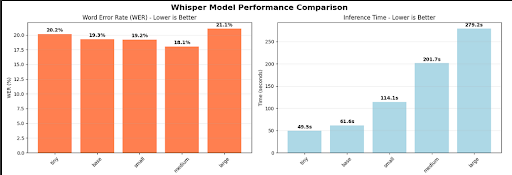
\includegraphics[scale = 0.9]{experiements/image/2 charts.png}
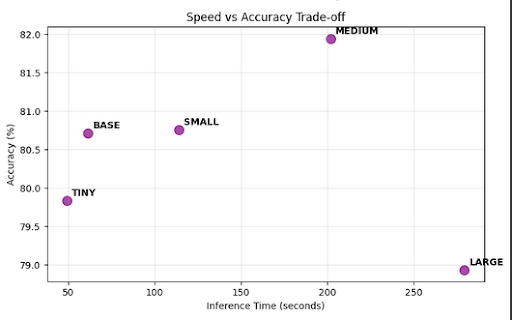
\includegraphics[scale = 0.8]{experiements/image/1 chart.png}
\\
\\
The evaluation demonstrates that \textbf{Whisper Small} is the most practical model for transcribing 30-minute academic lectures. It balances accuracy, runtime, and memory usage, making it well-suited for real-world deployment. Medium provides the highest accuracy but at prohibitive computational cost, while Tiny and Base sacrifice too much accuracy despite being efficient. Thus, for tasks such as summarization or real-time academic lecture processing, Whisper Small is recommended as the best-performing variant.